No es un secreto de que llevar a cabo una misión satelital representa grandes costos
y largos periódos de trabajo de desarrollo de la misión.
La NASA también padeció estos problemas hace algunas décadas.
Pero, al ser una organización que suele ir en contra de las corrientes y filosofías
normales de desarrollo, contar con personal altamente capacitado y disponer de recursos
económicos, pudo afrontar los obstáculos e innovar. Así, es como
surge su lema \textit{Faster, Better and Cheaper} (FBC).
El cual fue introducido por el administrador de la NASA Dan Goldin a
principios de la década de los 90's. Dan Goldin tenía una vasta experiencia en
el desarrollo de pequeños satélites, y estaba convencido de que el desarrollo
``clásico'' de misiones satelitales de NASA necesitaba un cambio de enfoque,
con el objetivo de lograr reducir el tiempo de desarrollo, y pasar de escala de tiempo de
décadas a años y, por sobre todo, lograr reducir costos \citep{Paxton07}.

Es sabido que el lema FBC produce una gran cantidad de fallas y
carencias en las misiones satelitales \citep{Paxton07}. Sin embargo,
esto es lo que impulsa la innovación, el desarrollo y entrenamiento de nuevos
managers, ingenieros y científicos, los cuales serán los líderes de las
nuevas generaciones \citep{Paxton07}. Por tales motivos, es importante,
que empresas y organizaciones del ámbito espacial en Argentina, dejen
de lado el ``clasicismo'', y se animen, y por supuesto, alienten a las futuras
generaciones, a transformar el tradicional \textit{caminar con los manuales de NASA bajo
  el brazo}. Lo cual implica volcarse al camino de la   innovación y el desarrollo
de nuevas tecnologías y técnicas para la realización de satélites (que en este trabajo se denominan
\textit{vehículos de nueva generación}). Esta visión fue adoptada por empresas tales como INVAP
y otras tanto nacionales como extranjeras,  que están creciendo a paso agigantados llevando
en su interior el cambio de filosofía que se exige, para lograr reducir costos, y 
alcanzar la capacidad necesaria para producir a gran escala.

El presente  trabajo tiene como objetivo demostrar que es posible desarrollar
vehículos espaciales utilizando componentes COTS de baja confiabilidad, trayendo
consigo una reducción considerable del costo y del tiempo de desarrollo. De más está
decir, que esta tesis no busca desarrollar en profundidad una arquitectura
que alcance los niveles de detalles que son esperables en una misión satelital, debido a que para
el cumplimiento de este objetivo se requiere de la colaboración interdisciplinar de equipos de 
ingenieros, managers y científicos. Si no, que el presente trabajo pretender servir como
base o puntapié inicial de líneas de investigación y desarrollo en el campo de estudio.
Debido a que como se demostró, es factible el desarrollo de arquitecturas
``económicas'', con la aplicación de técnicas y filosofías que van más allá de lo tradicional.

Luego de llevar a cabo un análisis de los sistemas satelitales y de aviónica que se
han publicado en diferentes trabajos de investigación, y como resultado de  diversas reuniones
con varios equipos dentro de la Unidad de Desarrollo INVAP, se llegó a la siguiente conclusión:
se debe promover el trabajo sobre el desarrollo de aviónicas aún cuando sus componentes
sean de baja confiabilidad, la comunicación entre componentes,
y que existe una tendencia a implementar redes de componentes dentro de los sistemas.

Una vez realizado este análisis previo, se estudiaron diferentes redes que tengan
la característica de ser tolerante a fallas y que sean factibles de ser
aplicadas en el ambiente espacial, como se indicó en la sección de Marco
Teórico (Capítulo \ref{chap:marco_teorico} Página \pageref{chap:marco_teorico}) y en
el Estado del Arte (Capítulo \ref{chap:estado_del_arte} Página \pageref{chap:estado_del_arte}).
Las cuales fueron las siguientes:
\begin{itemize}
\item Árboles binarios
\item Redes hypercube
\item Redes distribuídas
\end{itemize}

Los resultados del análisis de la confiabilidad se encuentra detallada en la sección
\ref{seccion:TopologiaEstudio} (Página \pageref{seccion:TopologiaEstudio}) y en
\cite{Arias17}. Resumiendo, como se puede observar en la Figura
\ref{fig:comparative_reliablitiesConclusion}, una vez realizada una comparativa
entre redes tolerantes a fallas, la que presenta un mayor grado
de confiabilidad sostenible en el tiempo es la que corresponde a
la red distribuida. Este resultado representa un importante aporte para el
conocimiento de tipos de topologías confiables tolerantes a fallas, y el desarrollo de
modelos para lograr medir la confiabilidad de esas topologías. Debido a que
permitirá reemplazar la estrucutra tradicional de un simple bus de comunicación, centralizada
en una On Board Computer (OBC), comúnmente la computadora del subsistema de C&DH
(Command and Data Handling), por una estructura distribuida, dónde no existen
rangos de importancia entre componentes,  sino que todas las computadoras
tiene la capacidad suficiente, y deben ejecutar las tareas de todos los subsistemas
de manera distribuida. 

\begin{comment}
Los resultados de
este estudio fueron presentados en el \textit{Congreso Argentino de Tecnologías
  Espaciales 2017 (Córdoba, Argentina)}
\end{comment}

\begin{figure}[H]
 \centering
 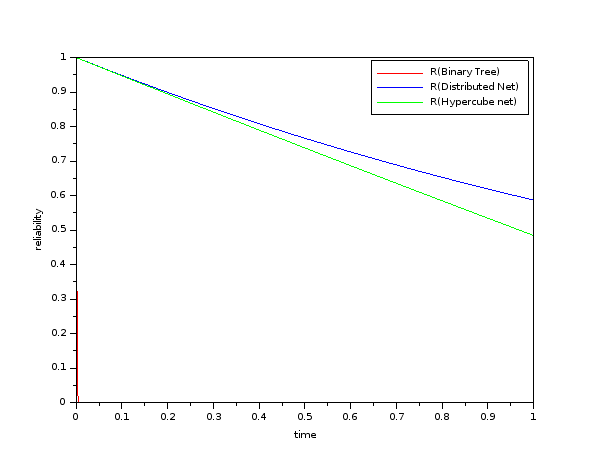
\includegraphics[scale=0.5]{images/Capitulo4/comparative_reliablities.png}
  \caption{Comparación de confiabilidad}
\label{fig:comparative_reliablitiesConclusion}
\end{figure}

Un requerimiento que fue planteado por la Unidad de Desarrollo INVAP fue trabajar
con el bus de comunicación CAN. Este es un protocolo de comunicación de bajo nivel,
que demuestra ser altamente confiable por lo que es utilizado en la industria automotriz,
que fue la promotora de su creación. Esto, nos da una clara razón de que CAN es un
protocolo confiable, debido a que en la fabricación de automóviles se tiene que cumplir
el objetivo de que el producto final no ponga en riesgo la vida de personas.
Además, por su confiabilidad, y a su excelente respuesta en sistemas de tiempo real,
CAN es utilizado también en el ambiente espacial (entre otras industrias), pero
relegado a ser un bus secundario.

En base a estos resultados y restricciones se plantea como un desafío a futuro implementar,
crear, diseñar, una arquitectura que sea capaz de trabajar con una filosofía
de red distribuida, la cual se encuentra descripta en la sección \ref{chap:arquitectura_propuesta}
(Página \pageref{chap:arquitectura_propuesta}). El grado de innovación que coloca
esta nueva arquitectura se ve reflejada en que no existe una computadora única (la
connotación ``única'' hace referencia a la computadora propiamente dicha más sus
redundancias, o bien, cualquier (micro)controlador más sus redundancias) por cada
subsistema como se trabaja ``tradicionalmente'' sino que, existen computadoras
híbridas capaces de llevar a cabo tareas de todos los sistemas en forma distribuida. 
Para ello se planteó un protocolo basado en CAN y CANOpen. Este protocolo, hasta el
momento, se encuentra en su versión 0.1 Alpha. El protocolo
presenta la innovación de estar orientado a objetos, y para ello se utilizó el
lenguaje SysML (System Modeling Language) para llevar a cabo su modelado y
la documentación del mismo. Esto facilita la interpretación del
stack de servicio que debe ser implementado a la hora del desarrollo. Este protocolo
se encuentra documentado en el apéndice \ref{Appendix:A} (Página \pageref{Appendix:A}).

En base a los resultados obtenidos y a la arquitectura propuesta basada en CANae
(apéndice \ref{Appendix:A}) se concluye de que es factible  desarrollar una
\textit{arquitectura de aviónica tolerantes a fallas basada en componentes COTS para
  vehículos satelitales} utilizando el bus CAN, como bus principal de comunicación.
Si bien esto exige un cambio de paradigma importante, los datos recolectados en el
presente trabajo demuestran que es posible diseñar arquitecturas
fiables basadas en componentes que sean baratos y de baja confiabilidad. 

\section{Conclusiones finales}
\begin{comment}
En la Tabla \ref{table:objetivos_cumplidos} se describe
si los objetivos planteados fueron cumplimentados o no.
\begin{table}[h!]
\small
\centering
\caption{Tabla de objetivos cumplidos}
\label{table:objetivos_cumplidos}
\begin{tabular}{|p{7cm}|p{8cm}|}
\hline
\multicolumn{1}{|c|}{\textbf{Objetivo planteado}} & \multicolumn{1}{c|}{\textbf{Resultado}} \\ \hline
El objetivo de este trabajo es investigar y analizar arquitecturas de comunicación de los subsistemas de
aviónica tolerante a fallas basada en componentes COTS para vehículos satelitales de nueva generación. & Cumplido \\ \hline
Realizar un estudio del estado de la cuestión sobre arquitecturas tolerantes a fallas para sistemas críticos. & Cumplido \\ \hline
Investigar y analizar arquitecturas tolerantes a fallas que aseguren la confiabilidad del sistema y que sean
aplicables en la industria satelital. & Cumplido \\ \hline
Investigar y analizar protocolos de comunicación, para las capas superiores del modelo de OSI (modelo
de interconexión de sistemas abiertos - ISO/IEC 7498-1), orientados a la tolerancia a fallas y confiabilidad
de los sistemas. Realizar un estudio comparativo de los diferentes protocolos estudiados. & No cumplido. Debido a la complejidad
del objetivo demandaría una cantidad de tiempo extra, y no alcanzaría para ser cumplido en el tiempo preestablecido. Se decidió
trabajar directamente con CAN. \\ \hline
Investigar una metodología para lograr una medición de la tolerancia a fallas en arquitecturas de aviónica & Cumplido. Se investigó
metodologías para la medición de topologías. \\ \hline
Desarrollar un estudio comparativo de arquitecturas tolerantes a fallas con el fin de obtener ventajas y
desventajas de cada una de ellas. & No cumplido. No se compararon arquitecturas completas debido a que no alcanzaría a ser
cumplido en el tiempo preestablecido. En contraposición se compararon topologías. \\ \hline
Diseñar modelos alternativos de arquitecturas tolerantes a fallas, que tenga un grado de confiabilidad tal
que permita la aplicación de componentes COTS. & No cumplido. Solo se desarrolló una arquitectura debido a cuestiones de tiempo. \\ \hline
Evaluar la confiabilidad de los modelos de arquitecturas (mediante métrica desarrollada en este trabajo o
siguiendo otras estrategias). & No cumplido. \\ \hline
Proponer el diseño de una nueva arquitectura tolerante a fallas, con un grado de confiabilidad suficiente
para la aplicación de componentes COTS en aviónicas de vehículos satelitales. & Cumplido. \\ \hline
Simular la arquitectura planteada para medir su grado de tolerancia a fallas y perfomance. & No cumplido. \\ \hline
\end{tabular}
\end{table}

En cuanto a las preguntas de investigación que se plantearon para este trabajo de tesis, las respuestas de estas
se describen a continuacion:

\begin{itemize}
\item \textbf{¿Es posible la realización de un método de medición del grado de tolerancia a fallas de una arquitectura
de aviónica?} \textit{No fue posible responder. Se logró desarrollar una manera de comparar la confiabilidad de 
topologías de arquitecturas, basándose en la tolerancia a fallas. }
\item \textbf{¿Cuál es la estrategia más indicada de tolerancia a fallas que permita brindar un alto grado de confiabili-
dad en la utilización de componentes COTS en sistemas críticos?} \textit{En este trabajo se demostró
que la estrategía más indicada es desarrollar una arquitectura basada en red distribuida.}
\item \textbf{¿Cuál es la arquitectura más indicada que permita desarrollar tolerancia a fallas en sistemas críticos
basados en componentes COTS?} \textit{La arquitectura basada en CANae desarrollada en este trabajo de tesis,
cumple con las necesidades necesarias para sentar las bases de trabajos futuros en la implementación de
arquitecturas confiables basadas en componentes COTS.}
\item \textbf{¿Es factible la utilización de componentes COTS en sistemas espaciales?} \textit{Este trabajo de tesis
demostró que es factible la utilización de componentes COTS.}
\end{itemize}
\end{comment}

En el presente trabajo de tesis se demostró que es factible la utilización de
componentes COTS en sistemas espaciales. Si bien, no se pudo responder si es
posible la realización de un método de medición del grado de tolerancia a
fallas de una arquitectura de aviónica, se logró desarrollar una manera
de comparar confiabilidad de topologías de arquitectura, basándose en la
tolerancia a fallas.

En este trabajo se demostró que la estrategia más indicada de tolerancia a
fallas que permite brindar un alto grado de confiabilidad en la utilización de
componentes COTS en sistemas críticos, es desarrollar una arquitectura basada en
una red distribuida, debido a que de esta manera se logra distribuir las tareas
entre todos las computadoras que conforman la arquitectura,
y ante cualquier eventualidad (o falla), la red se puede reconfigurar sencillamente,
y al no estar ligada una computadora a un subsistema (enfoque tradicional), las tareas
se redistribuyen dinámicamente sin perjudicar el funcionamiento normal
del sistema, en otras palabras aumenta a su tolerancia a fallas.

La arquitectura basada en CANae, demostró ser la arquitectura más indicada que permita
desarrollar tolerancia a fallas en sistemas críticos basados en componentes COTS,
debido a que cumple con los requisitos para sentar las bases de trabajos futuros
en la implementación de arquitecturas confiables basadas en componentes COTS. 

\section{Perspectivas a futuros}\label{chap:TrabajosFuturos}
A partir de análisis realizado en este trabajo de tesis, se logra ver el gran
potencial que existe en el estudio de arquitecturas de aviónicas tolerantes
a fallas, y de los componentes COTS introducidos en el sistema,
donde el producto esperado debe ser más confiable que los componentes
que la conforman.

Por estos motivos, a futuro se pretende continuar con las siguientes lineas de trabajo:
\begin{itemize}
\item Diseño detallado, desarrollo e implementación del protocolo CANae.
\item Diseño detallado de la arquitectura propuesta.
\item Estudio de nuevas técnicas de tolerancia a fallas aplicadas a los diferentes niveles
de detalle de las arquitecturas de aviónica.
\item Desarrollo de algoritmos de ruteo para la distribución de tareas en redes distribuidas.
\item Estudio de tecnología Wireless como medio de comunicación alternativo al cableado.
\end{itemize}

